\documentclass[12pt, letterpaper]{article}
\usepackage[margin=1in]{geometry}
\usepackage{mathptmx}
\usepackage{amsmath}
\usepackage{graphicx}
\usepackage{booktabs}
\usepackage[font={small,it}, justification=centering, labelfont=bf]{caption}
\usepackage{float}
\usepackage[skip=4pt]{parskip}
\usepackage{hyperref}
\hypersetup{colorlinks=true, linkcolor=blue, urlcolor=blue}
\usepackage{titlesec}
\titlespacing*{\section}{0pt}{8pt}{4pt}
\titlespacing*{\subsection}{0pt}{6pt}{2pt}
\usepackage{listings}
\usepackage{xcolor}

% Roman numeral section counter
\renewcommand{\thesection}{\Roman{section}}
\titleformat{\section}{\normalfont\bfseries\large}{\thesection.}{0.5em}{}

% Simple arabic numbering for subsections (1. 2. 3. not III.1)
\renewcommand{\thesubsection}{\arabic{subsection}}
\titleformat{\subsection}{\normalfont\bfseries}{\thesubsection.}{0.5em}{}

% Code listings styling
\lstset{
  language=Verilog,
  basicstyle=\ttfamily\small,
  keywordstyle=\color{blue},
  commentstyle=\color{gray},
  stringstyle=\color{red},
  breaklines=true,
  frame=single,
  backgroundcolor=\color{white}
}

\begin{document}

\begin{center}
  {\large \textbf{Report for CDA 3201L Lab \#5}}\\[2pt]
  {\large \textbf{Combinational Logic Design with Higher Level Devices}}\\[8pt]
  \begin{tabular}{ll}
    \textbf{Name:} Tuan Khang Phan & \textbf{UID:} 030382645 \\
    \textbf{Name:} Huu Phat Nguyen & \textbf{UID:} U46082380 \\
  \end{tabular}
\end{center}

\section{Introduction}

The purpose of this lab is to get familiar with higher level digital devices like decoders and multiplexers, and to see how hierarchical design makes building circuits easier. Instead of wiring up a bunch of individual logic gates, we can use ICs that already have multiple gates inside them, which saves time and reduces the number of chips on the breadboard. In this lab, we built a 4-to-1 multiplexer from basic gates (inverters, ANDs, ORs), then compared its output to a commercial 74LS153N multiplexer IC to make sure they behave the same way. We also wrote Verilog code for a 2-to-1 mux and used it to build a 4-to-1 mux hierarchically.

\section{Methods and Materials}

We used the following components and equipment:

\begin{itemize}
  \item 74LS04N inverter IC
  \item 74LS08N 2-input AND gate IC (x2)
  \item 74LS32N 2-input OR gate IC
  \item 74LS86N XOR gate IC
  \item 74LS153N dual 4-to-1 multiplexer IC
  \item Breadboard
  \item Jumper wires
  \item LED and resistor
  \item 5\,V DC power supply
\end{itemize}

We started by writing out the truth tables for the 2-to-1 and 4-to-1 multiplexers and then derived the SOP expressions from those tables. For the 4-to-1 mux, the SOP has four product terms, each with three inputs (two select lines and one data input). Since the 74LS08N only provides 2-input AND gates, we had to cascade two AND gates for each product term, which doubled the number of AND gates we needed. After building the AND portion, we used OR gates from the 74LS32N to combine the four product terms into a single output.

We wired up the 74LS153N in parallel with our custom mux so both received the exact same inputs and select lines. To compare the two outputs, we connected them to a 74LS86N XOR gate followed by an inverter from the 74LS04N. When both outputs match, the XOR gives 0, and the inverter flips it to 1, lighting up the LED. If the outputs ever disagree, the LED turns off.

For testing, we set the data inputs to $I_0 = 1$, $I_1 = 0$, $I_2 = 1$, $I_3 = 0$ (the pattern 1010) by connecting them to VDD or GND accordingly. Then we tried all four select line combinations and observed the LED.

For the Verilog part, we wrote a simple 2-to-1 mux module and instantiated it three times to build a 4-to-1 mux. We wrote a testbench to go through all possible combinations and checked the output.

\section{Results}

\subsection{Truth Table and Equations for Multiplexers}

For a 2-to-1 multiplexer with data inputs A and B and select line S:

\begin{center}
  \begin{tabular}{|c|c|}
    \hline
    S & Output \\
    \hline
    0 & A \\
    1 & B \\
    \hline
  \end{tabular}
\end{center}

The SOP expression is: $Y = \overline{S} \cdot A + S \cdot B$

For a 4-to-1 multiplexer with data inputs $I_0$, $I_1$, $I_2$, $I_3$ and select lines $S_1$ and $S_0$:

\begin{center}
  \begin{tabular}{|cc|c|}
    \hline
    $S_1$ & $S_0$ & Output \\
    \hline
    0 & 0 & $I_0$ \\
    0 & 1 & $I_1$ \\
    1 & 0 & $I_2$ \\
    1 & 1 & $I_3$ \\
    \hline
  \end{tabular}
\end{center}

The SOP expression is:
\[
Y = \overline{S_1} \cdot \overline{S_0} \cdot I_0 + \overline{S_1} \cdot S_0 \cdot I_1 + S_1 \cdot \overline{S_0} \cdot I_2 + S_1 \cdot S_0 \cdot I_3
\]

\subsection{Chip Count and Gate Analysis}

To build the 4-to-1 multiplexer from basic gates, we needed:

\begin{itemize}
  \item 2 inverters (from 74LS04N) to generate $\overline{S_0}$ and $\overline{S_1}$
  \item 8 two-input AND gates (from 2 x 74LS08N) because each of the 4 product terms requires 3 inputs, and with 2-input AND gates we need to cascade two per term
  \item 3 two-input OR gates (from 74LS32N) to combine the 4 product terms in a tree structure
\end{itemize}

For the comparator circuit, we used 1 XOR gate (from 74LS86N) and 1 additional inverter (from the same 74LS04N).

In total, the entire setup used 5 ICs for the custom mux and comparator: 1 x 74LS04N, 2 x 74LS08N, 1 x 74LS32N, 1 x 74LS86N. Plus the 74LS153N as the reference mux.

\subsection{Verilog Implementation}

The 2-to-1 multiplexer module:

\begin{lstlisting}
module mux_2to1(
  input A, B, S,
  output Y
);
  assign Y = (~S & A) | (S & B);
endmodule
\end{lstlisting}

The 4-to-1 multiplexer built from three 2-to-1 mux instances. The first two muxes each handle a pair of inputs using $S_0$ as the select, and the third mux picks between those two results using $S_1$:

\begin{lstlisting}
module mux_4to1(
  input I0, I1, I2, I3, S0, S1,
  output Y
);
  wire mux0_out, mux1_out;

  mux_2to1 U1(.A(I0), .B(I1), .S(S0), .Y(mux0_out));
  mux_2to1 U2(.A(I2), .B(I3), .S(S0), .Y(mux1_out));
  mux_2to1 U3(.A(mux0_out), .B(mux1_out), .S(S1), .Y(Y));
endmodule
\end{lstlisting}

The testbench cycles through all 64 possible combinations of the 6 inputs:

\begin{lstlisting}
module mux_4to1_tb();
  reg I0, I1, I2, I3, S0, S1;
  wire Y;
  integer i;

  mux_4to1 UUT(.I0(I0), .I1(I1), .I2(I2), .I3(I3),
               .S0(S0), .S1(S1), .Y(Y));

  initial begin
    $dumpfile("mux_test.vcd");
    $dumpvars;
    $display("Time\tS1 S0\tI0 I1 I2 I3\tY");
    $monitor("%3d\t%b  %b\t%b  %b  %b  %b\t%b",
             $time, S1, S0, I0, I1, I2, I3, Y);

    for (i = 0; i < 64; i = i + 1) begin
      {S1, S0, I0, I1, I2, I3} = i;
      #10;
    end
    $finish;
  end
endmodule
\end{lstlisting}

% TODO: Insert console output screenshot and waveform screenshot here
% \begin{figure}[H]
% \centering
% \includegraphics[width=0.95\linewidth]{console_output.jpg}
% \caption{Console output from the 4-to-1 mux testbench simulation.}
% \end{figure}

% \begin{figure}[H]
% \centering
% 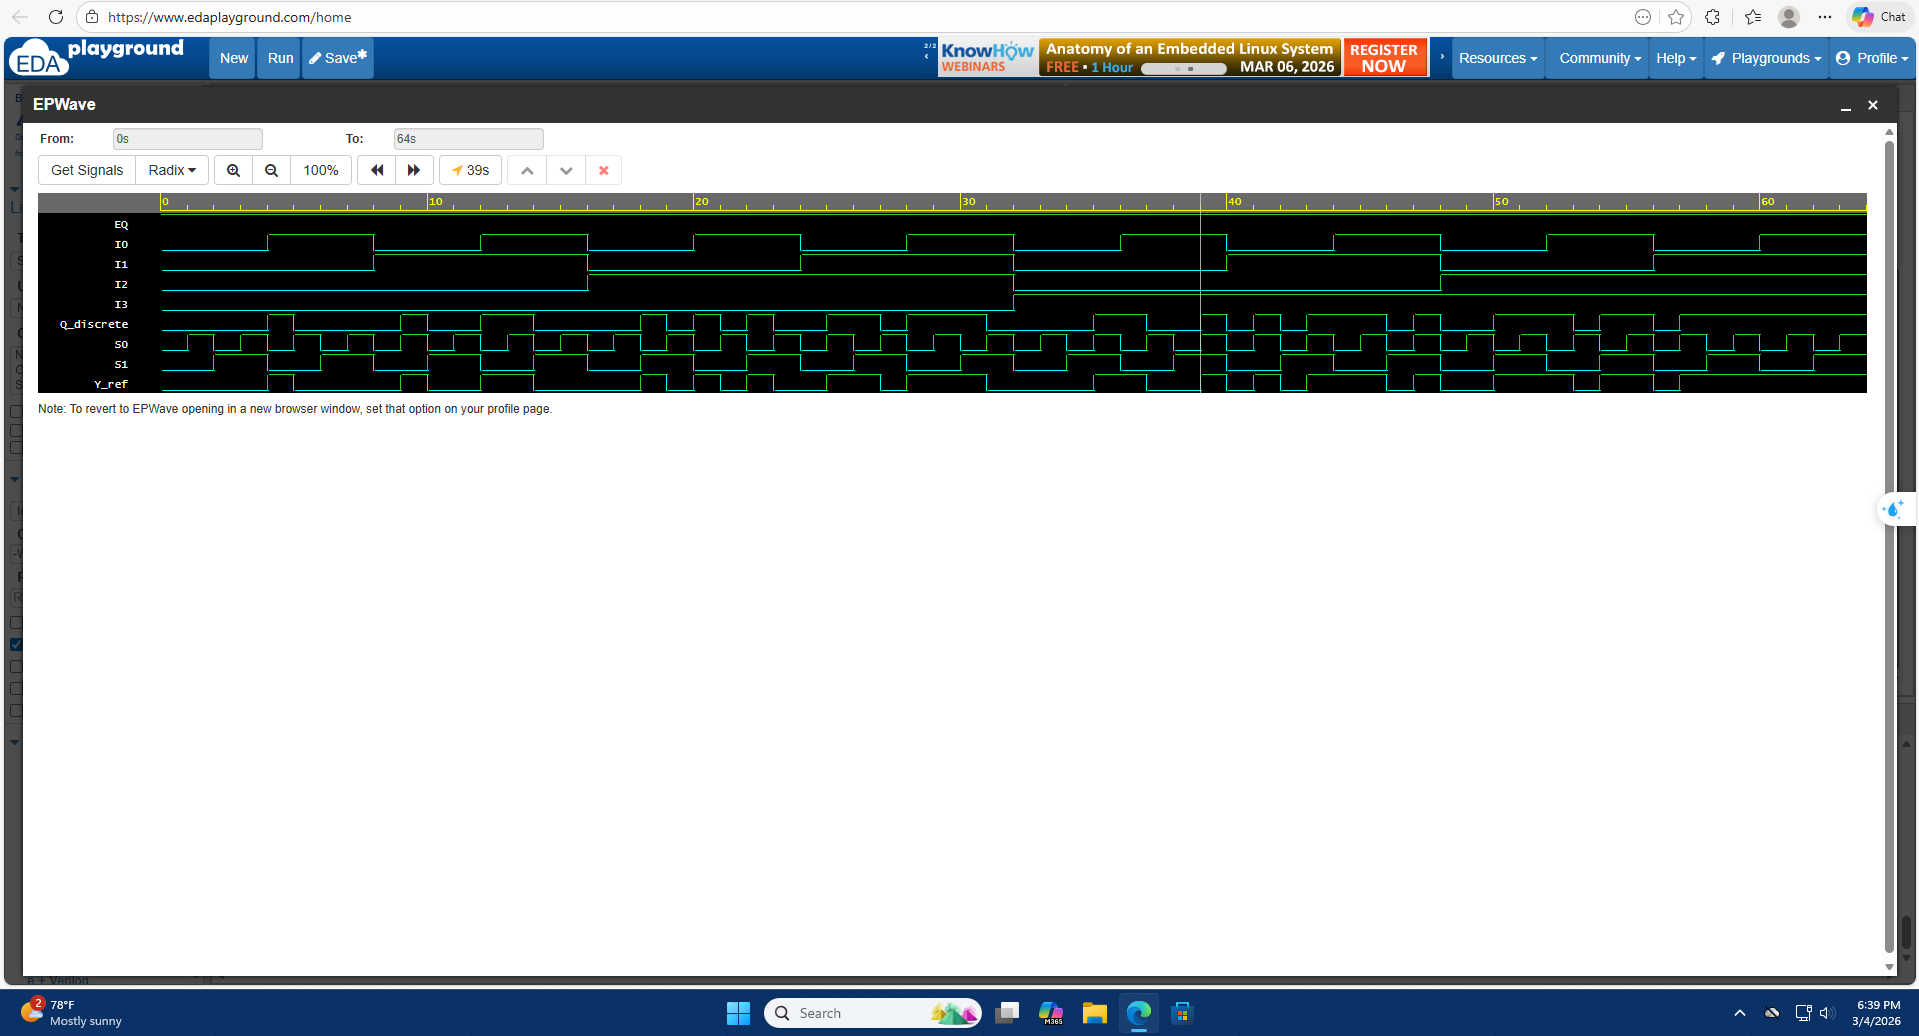
\includegraphics[width=0.95\linewidth]{waveform.jpg}
% \caption{Waveform from the 4-to-1 mux testbench simulation.}
% \end{figure}

\subsection{Physical Circuit Testing}

We set the data inputs to $I_0 = 1$, $I_1 = 0$, $I_2 = 1$, $I_3 = 0$ and tried each select combination. The results were:

\begin{center}
  \begin{tabular}{|cc|c|c|}
    \hline
    $S_1$ & $S_0$ & Expected Output & LED \\
    \hline
    0 & 0 & $I_0 = 1$ & ON \\
    0 & 1 & $I_1 = 0$ & OFF \\
    1 & 0 & $I_2 = 1$ & ON \\
    1 & 1 & $I_3 = 0$ & OFF \\
    \hline
  \end{tabular}
\end{center}

The LED turned on for $S_1S_0 = 00$ and $S_1S_0 = 10$, and stayed off for $S_1S_0 = 01$ and $S_1S_0 = 11$. This matches exactly what we expected since $I_0$ and $I_2$ are tied to HIGH while $I_1$ and $I_3$ are tied to LOW. Both our custom mux and the 74LS153N produced the same output for every combination we tested.

\begin{figure}[H]
\centering
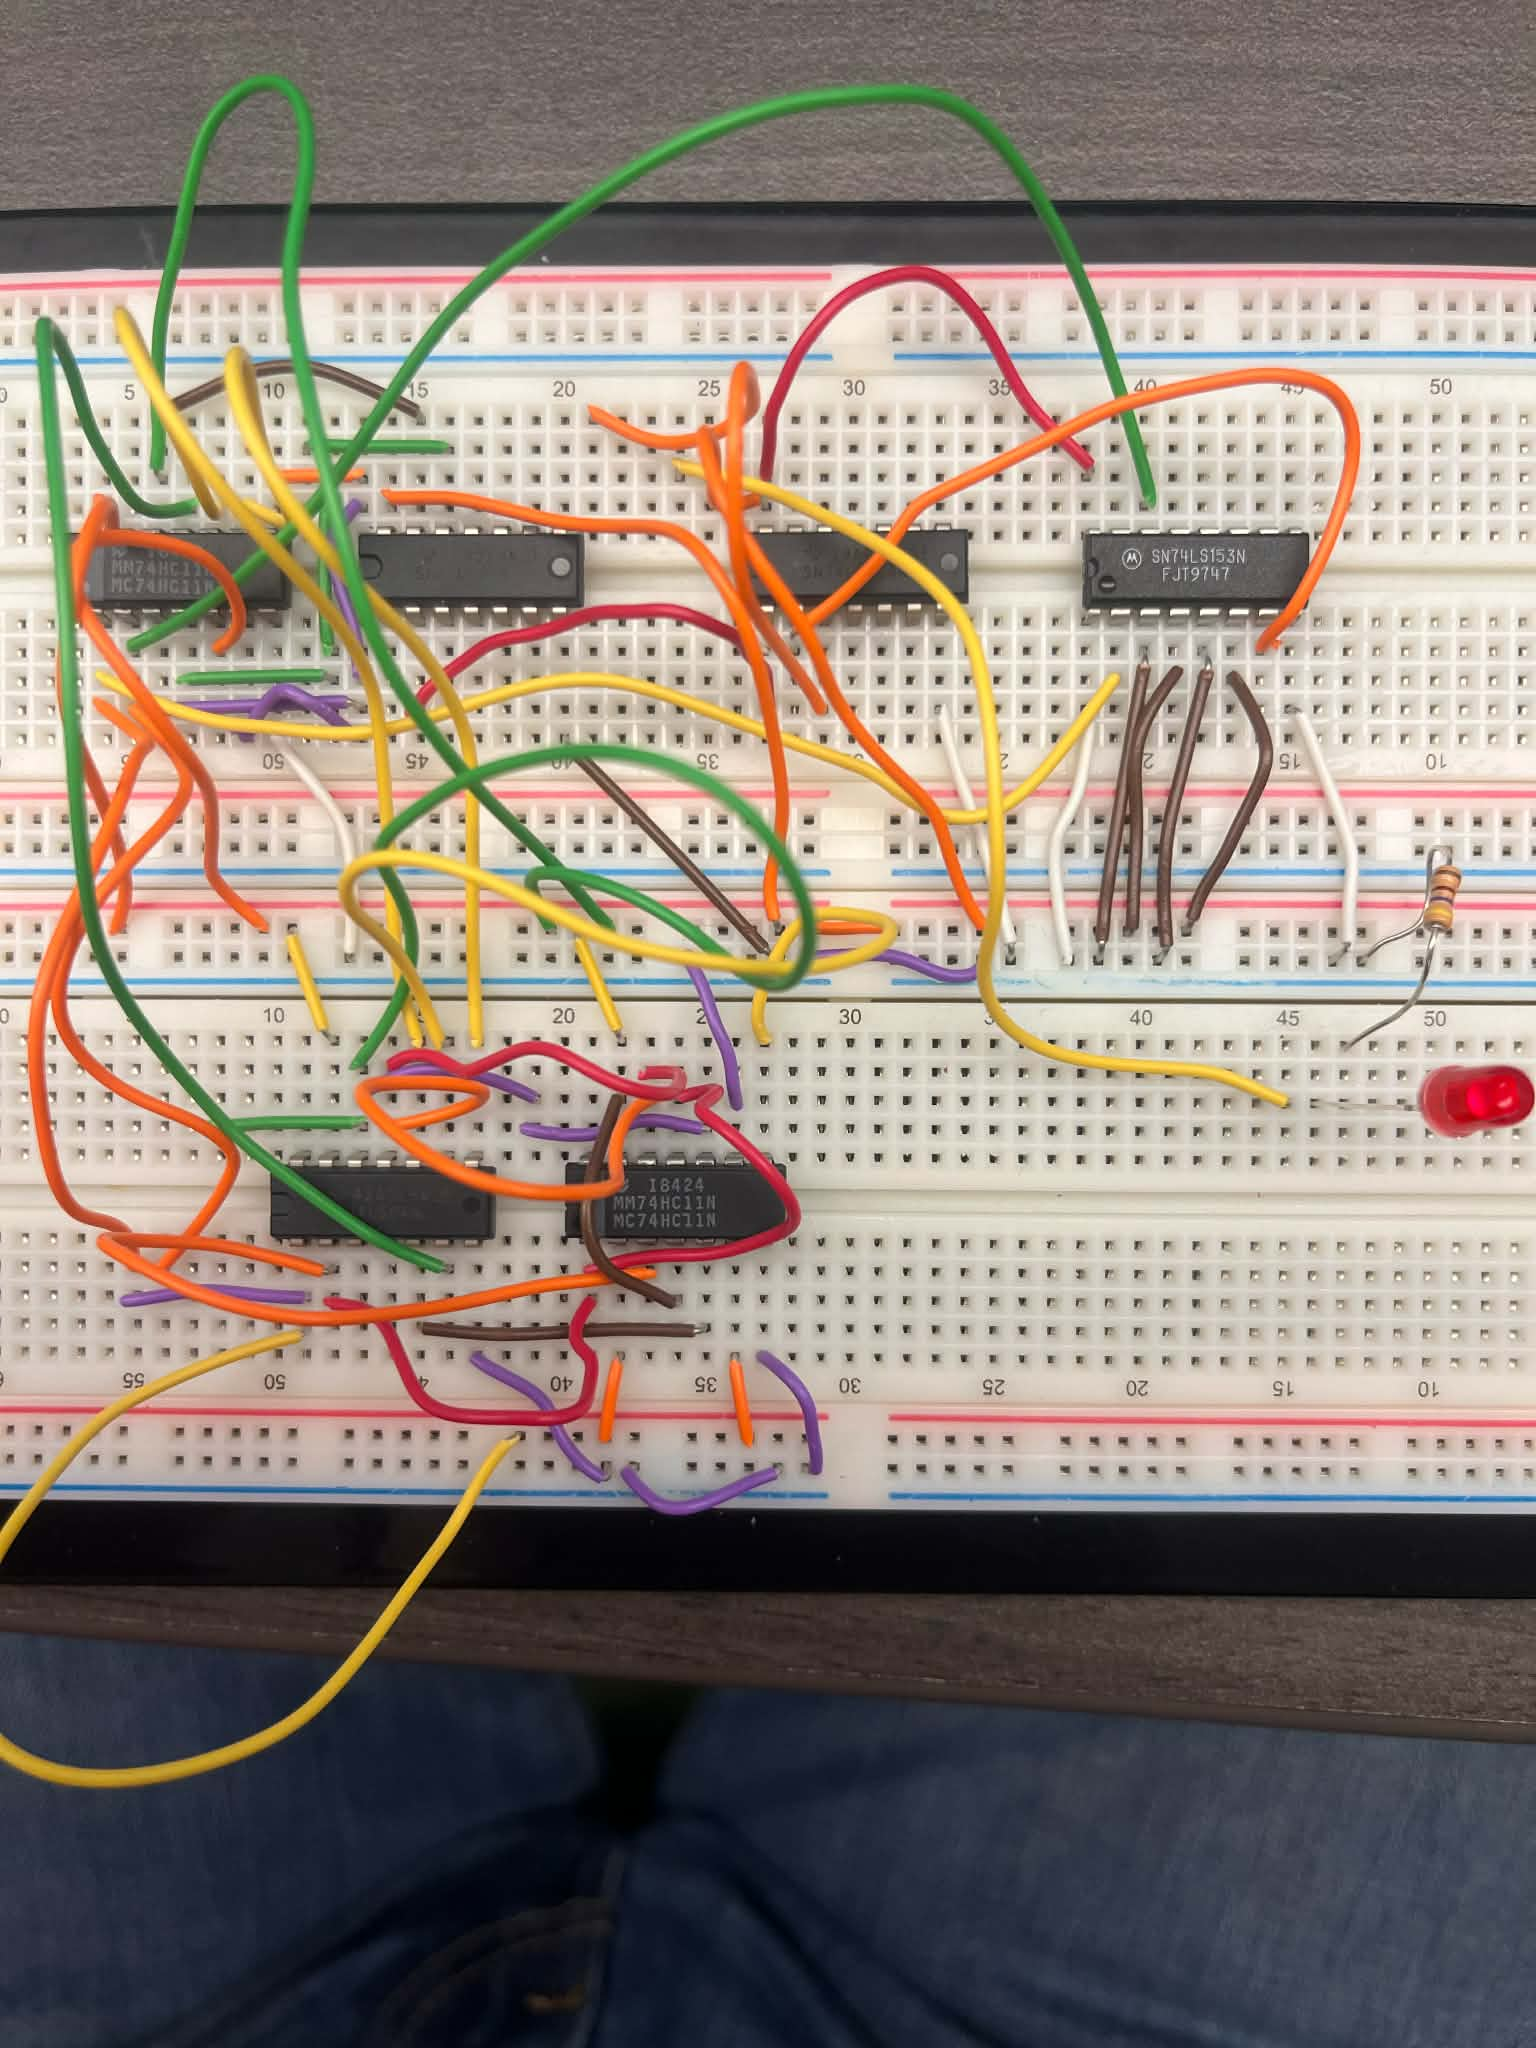
\includegraphics[width=0.85\linewidth]{cda_lab5_1.jpg}
\caption{Breadboard implementation of the 4-to-1 multiplexer circuit.}
\end{figure}

\begin{figure}[H]
\centering
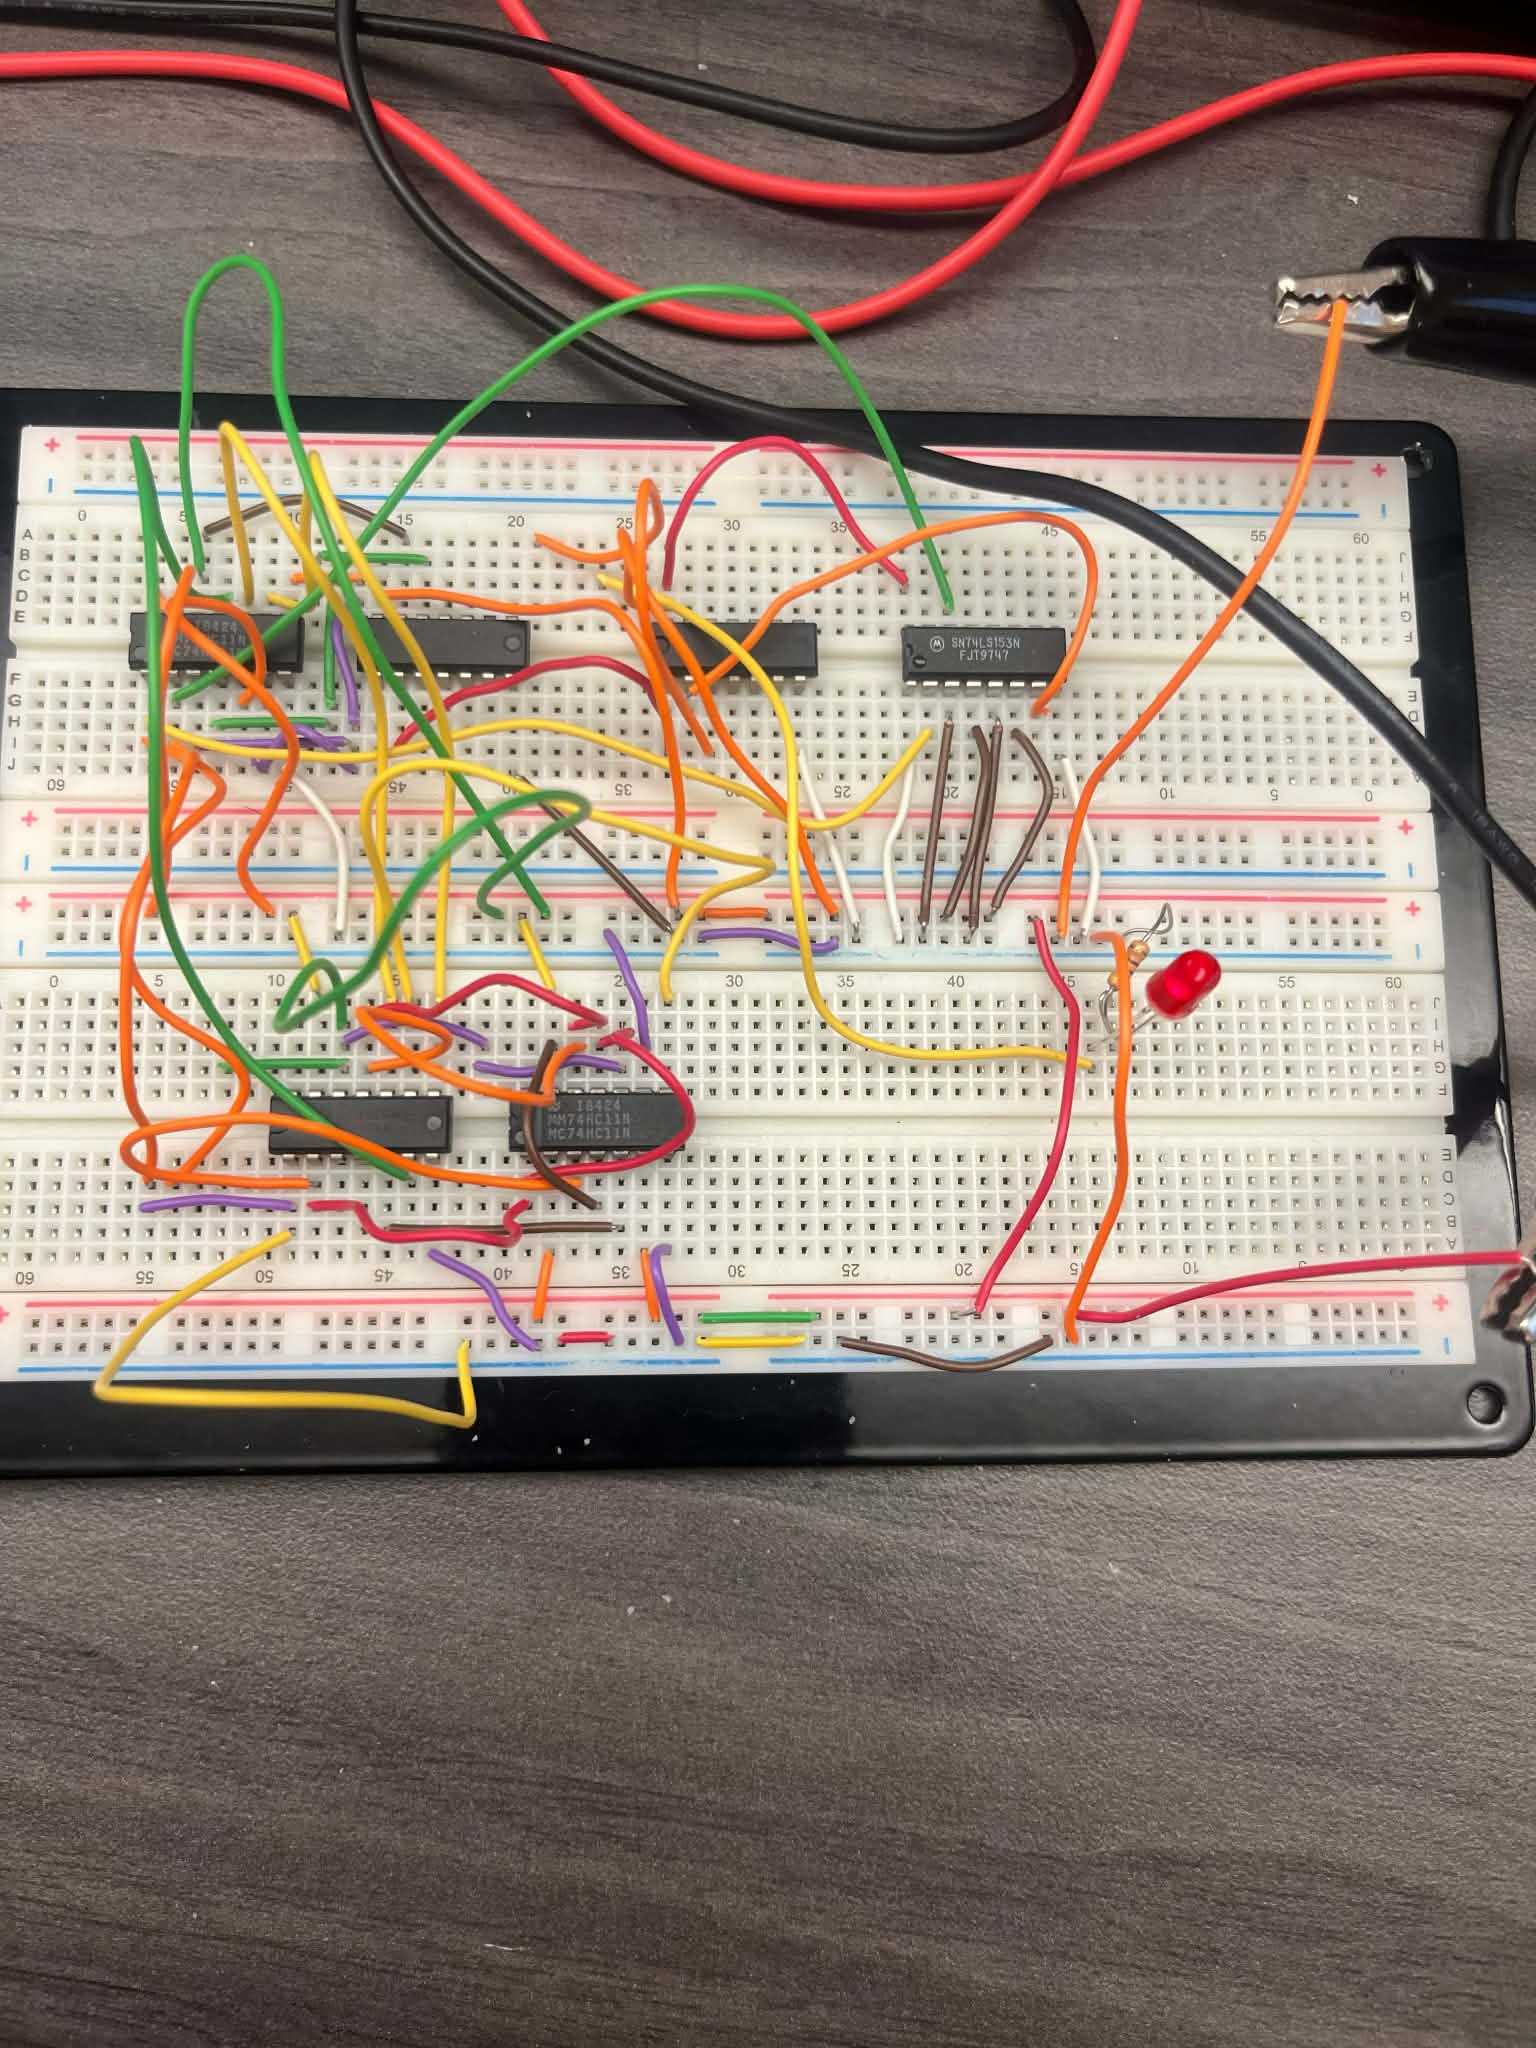
\includegraphics[width=0.85\linewidth]{cda_lab5_2.jpg}
\caption{Testing setup with both the custom mux and the 74LS153N connected in parallel.}
\end{figure}

\section{Lab Assignment Questions}

\subsection{Why is hierarchical design important?}

Hierarchical design lets us break a big circuit into smaller pieces that are easier to build and test on their own. In Verilog, for example, we wrote a simple 2-to-1 mux and reused it three times to make a 4-to-1 mux. If one of those sub-modules has a bug, we can test it in isolation instead of debugging the whole thing at once. On the physical side, using ICs like the 74LS153N means we do not have to wire up dozens of individual gates, which saves breadboard space and reduces wiring mistakes.

The main benefit is reusability. Once a sub-module is tested and working, you can use it in many different designs without starting from scratch. The potential drawback is that a hierarchical design might not be as optimized as a flat one. For instance, building a 4-to-1 mux from three 2-to-1 muxes uses more gates than the minimum SOP implementation. There is also a learning curve when it comes to understanding how all the modules connect together, especially in larger designs.

\subsection{Using decoders to realize SOP functions}

With an active HIGH decoder, each output corresponds to exactly one minterm. To implement any SOP function, we just OR together the decoder outputs for the minterms we need. For example, if $f(a,b,c) = \sum m(5,6,7)$, we connect outputs 5, 6, and 7 of a 3-to-8 decoder to an OR gate. We can even implement multiple functions from the same decoder by using different OR gates connected to different subsets of outputs.

With an active LOW decoder (where the selected output goes to 0 and all others stay at 1), we use NAND gates instead of OR gates to combine the desired minterms. This works because NANDing the active low outputs is logically equivalent to ORing active high outputs.

The main limitation is fan-out. Each decoder output can only drive a certain number of gate inputs before the signal degrades. If we try to connect one output to too many OR or NAND gates for different functions, it may exceed the drive strength of that output. Also, for functions with many variables, the decoder size grows exponentially ($2^n$ outputs for $n$ inputs), which becomes impractical for large $n$.

\subsection{Constructing an 8-to-1 mux from 4-to-1 muxes}

We would use two 4-to-1 muxes and one 2-to-1 mux. The first 4-to-1 mux takes inputs $I_0$ through $I_3$ and uses $S_0$ and $S_1$ as its select lines. The second 4-to-1 mux takes inputs $I_4$ through $I_7$ with the same $S_0$ and $S_1$ select lines. Then the outputs of these two muxes go into a 2-to-1 mux that uses $S_2$ as its select line. When $S_2 = 0$, the output comes from the first group (inputs 0 through 3), and when $S_2 = 1$, it comes from the second group (inputs 4 through 7). This gives us a complete 8-to-1 selection with three select bits.

\section{Discussion}

The physical circuit worked as expected. With inputs set to 1010, the LED correctly turned on only when the selected input was HIGH ($S_1S_0 = 00$ selecting $I_0 = 1$ and $S_1S_0 = 10$ selecting $I_2 = 1$). The fact that both our custom mux and the 74LS153N agreed on every test case confirms that our gate level implementation of the SOP expression is correct.

One thing we noticed during the build is that the custom mux takes up a lot more space on the breadboard compared to just using the 74LS153N. We needed two 74LS08N chips because each product term requires a 3-input AND, but the 74LS08N only has 2-input gates, so we had to cascade them. This is a good example of why higher level ICs exist: they save board space, reduce wiring complexity, and are less prone to mistakes.

The Verilog implementation was straightforward once we had the 2-to-1 mux working. The hierarchical approach made it easy to scale up, and the testbench confirmed the output matched expectations for all 64 input combinations.

\section{Conclusion}

In this lab, we built a 4-to-1 multiplexer from basic logic gates and verified it against a 74LS153N IC. The two circuits produced identical results for every input combination we tested. We also implemented the same multiplexer hierarchically in Verilog using 2-to-1 mux modules. This lab showed us how higher level devices and hierarchical design simplify both physical and HDL based circuit implementation, and why these approaches are preferred over building everything from individual gates.

\end{document}
